\documentclass[12pt]{article}
\usepackage[margin=1in]{geometry}
\usepackage{amsmath}
\usepackage{amssymb}
\usepackage{tikz}
\usepackage{xcolor}
\usepackage{tcolorbox}
\usepackage{enumitem}

\definecolor{subcolor}{RGB}{0,102,204}
\definecolor{incomecolor}{RGB}{204,0,102}
\definecolor{totalcolor}{RGB}{0,153,51}

\title{\textbf{Slutsky Decomposition: A Clear Explanation}}
\author{ECO 310 Midterm Review}
\date{}

\begin{document}
\maketitle

\section*{The Big Picture}

When the price of a good changes, your consumption of that good changes. But \textbf{WHY} does it change? The Slutsky decomposition shows that there are \textbf{TWO DISTINCT REASONS}:

\begin{tcolorbox}[colback=blue!5!white,colframe=blue!75!black,title=The Two Effects]
\begin{enumerate}[leftmargin=*]
\item \textbf{\textcolor{subcolor}{Substitution Effect}}: The good became relatively more/less expensive compared to other goods, so you substitute toward the relatively cheaper good
\item \textbf{\textcolor{incomecolor}{Income Effect}}: Your real purchasing power changed (you're effectively richer or poorer), so you consume more/less of the good
\end{enumerate}
\end{tcolorbox}

\section{The Key Insight}

Imagine the price of coffee rises from \$2 to \$4 per cup, and you reduce your consumption from 10 cups to 4 cups per week. The total change is $-6$ cups. But this $-6$ comes from:

\begin{itemize}
\item \textbf{\textcolor{subcolor}{Substitution}}: Coffee is now twice as expensive relative to tea. Even if I gave you enough money to maintain your original satisfaction level, you'd still buy less coffee and more tea. Say you'd buy 7 cups instead of 10. That's $-3$ cups due to substitution.

\item \textbf{\textcolor{incomecolor}{Income effect}}: The price increase makes you effectively poorer. With your original budget, you can't afford as much. This poverty effect makes you buy even less coffee, from 7 cups down to 4 cups. That's another $-3$ cups due to the income effect.
\end{itemize}

\textbf{Total change} = \textcolor{subcolor}{Sub effect} + \textcolor{incomecolor}{Income effect} = $(-3) + (-3) = -6$

\section{The Formula}

\begin{tcolorbox}[colback=green!5!white,colframe=green!75!black,title=Slutsky Decomposition]
When price $p_1$ changes from $p_1$ to $p_1'$:

\vspace{0.3cm}

\textbf{Total Effect} = \textcolor{totalcolor}{$\Delta x_1^{\text{total}}$} = $x_1^{\text{new}} - x_1^{\text{original}}$

\vspace{0.2cm}

This equals:

\vspace{0.2cm}

\textcolor{subcolor}{\textbf{Substitution Effect}} = $x_1^{\text{compensated}} - x_1^{\text{original}}$

\quad + \textcolor{incomecolor}{\textbf{Income Effect}} = $x_1^{\text{new}} - x_1^{\text{compensated}}$
\end{tcolorbox}

\section{Step-by-Step Recipe}

\subsection*{Step 1: Find the Original Bundle}

At the initial prices $(p_1, p_2)$ and income $m$, solve the consumer's utility maximization problem:
\begin{align*}
\max_{x_1, x_2} \quad & u(x_1, x_2) \\
\text{s.t.} \quad & p_1 x_1 + p_2 x_2 = m
\end{align*}

This gives you the \textbf{original bundle} $(x_1^*, x_2^*)$ and \textbf{original utility} $\bar{u} = u(x_1^*, x_2^*)$.

\subsection*{Step 2: Find the Compensated Bundle}

The price changes to $(p_1', p_2)$. Now imagine we \textit{compensate} the consumer by giving them just enough extra money so they can still \textit{afford} their original utility $\bar{u}$ at the new prices.

Solve the expenditure minimization problem:
\begin{align*}
\min_{x_1, x_2} \quad & p_1' x_1 + p_2 x_2 \\
\text{s.t.} \quad & u(x_1, x_2) = \bar{u}
\end{align*}

Or equivalently, find the bundle on the original indifference curve where $MRS = \frac{p_1'}{p_2}$.

This gives you the \textbf{compensated bundle} $(x_1^c, x_2^c)$.

\subsection*{Step 3: Find the New Bundle}

Now solve the regular utility maximization at the new prices with the \textit{original} income $m$:
\begin{align*}
\max_{x_1, x_2} \quad & u(x_1, x_2) \\
\text{s.t.} \quad & p_1' x_1 + p_2 x_2 = m
\end{align*}

This gives you the \textbf{new bundle} $(x_1^{new}, x_2^{new})$.

\subsection*{Step 4: Calculate the Effects}

\begin{tcolorbox}[colback=yellow!10!white,colframe=orange!75!black]
\textcolor{subcolor}{\textbf{Substitution Effect:}}
\[x_1^{\text{SE}} = x_1^c - x_1^*\]

\textcolor{incomecolor}{\textbf{Income Effect:}}
\[x_1^{\text{IE}} = x_1^{new} - x_1^c\]

\textcolor{totalcolor}{\textbf{Total Effect:}}
\[x_1^{\text{TE}} = x_1^{new} - x_1^* = x_1^{\text{SE}} + x_1^{\text{IE}}\]
\end{tcolorbox}

\section{Key Properties}

\begin{enumerate}[leftmargin=*]
\item \textbf{Substitution Effect Sign:}
\begin{itemize}
\item Always moves in the \textbf{opposite direction} of the price change
\item If $p_1$ rises: \textcolor{subcolor}{$x_1^{\text{SE}} \leq 0$} (buy less)
\item If $p_1$ falls: \textcolor{subcolor}{$x_1^{\text{SE}} \geq 0$} (buy more)
\end{itemize}

\item \textbf{Income Effect Sign:}
\begin{itemize}
\item Depends on whether the good is \textbf{normal} or \textbf{inferior}
\item \textbf{Normal good:} When effectively poorer, buy less
  \begin{itemize}
  \item If $p_1$ rises (poorer): \textcolor{incomecolor}{$x_1^{\text{IE}} < 0$}
  \item If $p_1$ falls (richer): \textcolor{incomecolor}{$x_1^{\text{IE}} > 0$}
  \end{itemize}
\item \textbf{Inferior good:} When effectively poorer, buy more
  \begin{itemize}
  \item If $p_1$ rises (poorer): \textcolor{incomecolor}{$x_1^{\text{IE}} > 0$}
  \item If $p_1$ falls (richer): \textcolor{incomecolor}{$x_1^{\text{IE}} < 0$}
  \end{itemize}
\end{itemize}

\item \textbf{Total Effect:} Sum of the two effects. For normal goods:
\begin{itemize}
\item Both effects work in same direction
\item Price rises $\Rightarrow$ quantity demanded falls
\end{itemize}

\item \textbf{Giffen Good:} An inferior good where the income effect dominates
\begin{itemize}
\item $|x_1^{\text{IE}}| > |x_1^{\text{SE}}|$
\item Price rises but quantity demanded rises too!
\item Very rare in practice
\end{itemize}
\end{enumerate}

\newpage

\section{Graphical Interpretation}

Consider a price increase for good 1:

\begin{center}
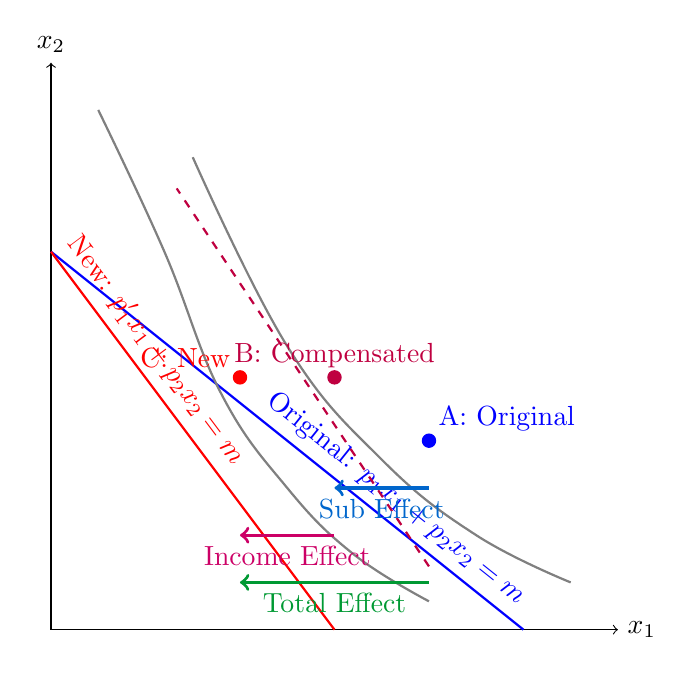
\begin{tikzpicture}[scale=1.2]
% Axes
\draw[->] (0,0) -- (6,0) node[right] {$x_1$};
\draw[->] (0,0) -- (0,6) node[above] {$x_2$};

% Original budget line (steeper)
\draw[thick, blue] (5,0) -- (0,4) node[pos=0.3, above, sloped] {Original: $p_1 x_1 + p_2 x_2 = m$};

% New budget line (flatter - good 1 is more expensive)
\draw[thick, red] (3,0) -- (0,4) node[pos=0.7, above, sloped] {New: $p_1' x_1 + p_2 x_2 = m$};

% Compensated budget line (parallel to new, tangent to old IC)
\draw[thick, purple, dashed] (4,0.67) -- (1.33,4.67);

% Indifference curves
\draw[thick, gray] plot[smooth, tension=0.7] coordinates {(5.5,0.5) (4.5,1) (3.5,1.8) (2.5,3) (1.5,5)};
\draw[thick, gray] plot[smooth, tension=0.7] coordinates {(4,0.3) (3.2,0.8) (2.5,1.5) (1.8,2.5) (1.2,4) (0.5,5.5)};

% Points
\filldraw[blue] (4,2) circle (2pt) node[above right] {A: Original};
\filldraw[purple] (3,2.67) circle (2pt) node[above] {B: Compensated};
\filldraw[red] (2,2.67) circle (2pt) node[above left] {C: New};

% Arrows showing effects
\draw[->, very thick, subcolor] (4,1.5) -- (3,1.5) node[midway, below] {Sub Effect};
\draw[->, very thick, incomecolor] (3,1) -- (2,1) node[midway, below] {Income Effect};
\draw[->, very thick, totalcolor] (4,0.5) -- (2,0.5) node[midway, below] {Total Effect};

\end{tikzpicture}
\end{center}

\textbf{Interpretation:}
\begin{itemize}
\item \textbf{Point A $\to$ Point B} (\textcolor{subcolor}{Substitution Effect}): Move along the original indifference curve to the new price ratio. The consumer substitutes away from the now-relatively-expensive good 1.

\item \textbf{Point B $\to$ Point C} (\textcolor{incomecolor}{Income Effect}): Remove the compensation. The consumer moves to a lower indifference curve because they're effectively poorer. For a normal good, they buy less of both goods.

\item \textbf{Point A $\to$ Point C} (\textcolor{totalcolor}{Total Effect}): The observed change in consumption.
\end{itemize}

\section{Special Cases}

\subsection*{Perfect Complements: $u = \min\{ax_1, bx_2\}$}

\textbf{Substitution Effect = 0}

With perfect complements, you always consume at the kink where $ax_1 = bx_2$. When the price changes, the compensated bundle has the exact same quantities as the original bundle (just on a different budget line). There's no substitution!

\textbf{Income Effect = Total Effect}

The entire change in consumption is due to the income effect.

\subsection*{Quasilinear: $u = v(x_1) + x_2$}

\textbf{Income Effect = 0} (for $x_1$ at interior solutions)

The optimal $x_1$ depends only on the price ratio, not on income. So the income effect for good 1 is zero!

\textbf{Substitution Effect = Total Effect}

The entire change in $x_1$ consumption is due to the substitution effect.

\section{Concrete Example}

\textbf{Setup:} $u = x_1 x_2$, $m = 100$, $p_2 = 1$, $p_1$ rises from 1 to 2.

\textbf{Step 1: Original Bundle}

With $p_1 = 1, p_2 = 1, m = 100$:
\begin{align*}
x_1^* &= \frac{m}{2p_1} = \frac{100}{2} = 50 \\
x_2^* &= \frac{m}{2p_2} = \frac{100}{2} = 50 \\
\bar{u} &= 50 \times 50 = 2500
\end{align*}

\textbf{Step 2: Compensated Bundle}

Need $x_1 x_2 = 2500$ and $MRS = \frac{x_2}{x_1} = \frac{p_1'}{p_2} = \frac{2}{1} = 2$.

From $\frac{x_2}{x_1} = 2$, we get $x_2 = 2x_1$.

Substituting into $x_1 x_2 = 2500$:
\[x_1 \cdot 2x_1 = 2500 \implies x_1^c = \sqrt{1250} \approx 35.36\]
\[x_2^c = 2x_1^c \approx 70.71\]

\textbf{Step 3: New Bundle}

With $p_1' = 2, p_2 = 1, m = 100$:
\begin{align*}
x_1^{new} &= \frac{m}{2p_1'} = \frac{100}{4} = 25 \\
x_2^{new} &= \frac{m}{2p_2} = \frac{100}{2} = 50
\end{align*}

\textbf{Step 4: Calculate Effects}

\begin{align*}
\text{\textcolor{subcolor}{Substitution Effect:}} \quad & x_1^c - x_1^* = 35.36 - 50 = \textcolor{subcolor}{-14.64} \\
\text{\textcolor{incomecolor}{Income Effect:}} \quad & x_1^{new} - x_1^c = 25 - 35.36 = \textcolor{incomecolor}{-10.36} \\
\text{\textcolor{totalcolor}{Total Effect:}} \quad & x_1^{new} - x_1^* = 25 - 50 = \textcolor{totalcolor}{-25}
\end{align*}

\textbf{Check:} $-14.64 + (-10.36) = -25$ \checkmark

\textbf{Interpretation:} When coffee price doubled, you reduced consumption from 50 to 25 cups. About 59\% of this reduction ($-14.64$) was due to substitution toward tea, and 41\% ($-10.36$) was due to being effectively poorer.

\section{Summary Checklist}

\begin{tcolorbox}[colback=green!5!white,colframe=green!50!black,title=Quick Reference]
\begin{itemize}[leftmargin=*]
\item \textbf{Three bundles:} Original, Compensated, New
\item \textbf{Compensated bundle:} Stay on original IC, move to new price ratio
\item \textbf{Sub effect:} Always opposes price change ($\leq 0$ if price rises)
\item \textbf{Income effect:} Depends on normal/inferior
\item \textbf{Normal good:} Both effects same direction when price changes
\item \textbf{Perfect complements:} Sub effect = 0
\item \textbf{Quasilinear:} Income effect = 0 (for $x_1$)
\item \textbf{Total = Sub + Income} always!
\end{itemize}
\end{tcolorbox}

\end{document}
